\documentclass[conference]{IEEEtran}
\usepackage{times}
\usepackage{epsfig}
\usepackage{graphicx}
\usepackage{amsmath}
\usepackage{amssymb}
\usepackage{multirow}
\usepackage[utf8]{inputenc}
\usepackage{stfloats}
\usepackage{afterpage}
\usepackage[breaklinks=true,bookmarks=false]{hyperref}

\begin{document}

\title{Deep Learning MRI Analysis for Automated Knee Injury Diagnosis}
\author{\IEEEauthorblockN{1\ Snehal Patil}
\IEEEauthorblockA{snehalpatil9914@gmail.com}
\and
\IEEEauthorblockN{2\ Supriya Alavala}
\IEEEauthorblockA{supriya.sportstar@gmail.com}
\and
\IEEEauthorblockN{3\ Ambar Gharat}
\IEEEauthorblockA{ambargharat2.0@gmail.com}
\and
\IEEEauthorblockN{4\ Akshath Kamath}
\IEEEauthorblockA{akshathkamathwork@gmail.com}
}

\maketitle

\begin{abstract}
   Improving the accuracy with which automated methods can identify injuries in
   MRIs of the knee would lead to time and cost savings for doctors and patients.
 By combining a set of transfer learning models utilizing pretrained neural networks for feature extraction and employing a blend of max pooling and attention mechanisms to integrate features from various frames within the MRI scan, we can achieve advancements beyond the existing leading performance on the MRNet challenge dataset.
\end{abstract}

\section{Introduction} 

Magnetic resonance imaging (MRI) is a method of obtaining three dimensional images of the inside of an object by using strong magnets to align the protons in the object and then radio frequency currents to disrupt and measure that alignment. An MRI sequence is a series of two dimensional images that can be stacked to recreate the three dimensional object. There are three sequence types, each corresponding to an orientation of the ``camera'' that captures the two dimensional slices. The axial sequence captures slices of the object that are horizontal to the ground; the coronal sequence captures vertical slices as viewed from the front of the object; and the sagittal sequence captures vertical slices as viewed from the side of the object.

MRI can be a useful tool when diagnosing knee injuries\cite{orlando2015diagnosis,figueiredo2018use,smith2012diagnostic}, however, analyzing the images is a time-consuming process and, even with trained professionals, it is easy for a clinician to misdiagnose an injury based on an MRI reading\cite{kolata2011}. Improving the automated identification of abnormalities in knee MRIs could help prioritize which MRIs to examine first, as well as provide better early results for patients whose scans appear normal. Model predictions could also provide a ``second opinion'' which would reduce the possibility of missed abnormalities. This could represent a large cost savings for hospitals and an increased level of care for patients.

The issue addressed in this paper pertains to the following scenario: given a set of three MRI sequences (axial, coronal, and sagittal) of a patient's knee, can we forecast the existence of conditions necessitating surgical intervention? Specifically, our aim is to anticipate whether the knee exhibits normal health, manifests an ACL injury, shows indications of a meniscus injury, or presents with any other irregularity. Since these conditions may coincide, our objective is to predict three distinct binary outcomes: irregularity, ACL rupture, and meniscus impairment. Previous research has established that MRI scans serve as precise and sensitive diagnostic tools for identifying these types of ailments in a non-invasivemanner.manner\cite{boeve1991magnetic,felli2016comparison,yaqoob2015diagnostic}.


\section{Related work}
\label{related-work} 

There are two main challenges when trying to use automated methods on MRI sequences. The first is that each MRI scan has high information content because it is a 3-dimensional image of the patient. Determining how to extract meaning from a variable length series of images is non-trivial. Complicating things further, the second challenge is that MRIs are difficult and expensive to collect, which means that MRI data sets are too small for most deep learning approaches. Deep learning models must be constrained to a limited number of parmeters and updates to prevent overfitting.

Most recent deep learning MRI work deals with the 3-dimensional nature of MRI images by using 3D-CNNs, which take the idea of $(channel, width, height)$ convolutions that are swept across a 2-dimensional image and extends them to $(time, channel, width, height)$ convolutions that are swept across the 3-dimensional scan
\cite{hosseini2016alzheimer,wei2018flair,khvostikov20183d,zou20173d}. 
However, these models face constraints due to the substantial parameter count essential for 3D-CNNs and the necessity for training them anew.






Another common method is the so-called 2.5D approach, where models are trained on sliding windows of the input sequence \cite{roth2015improving,alkadi20182,grovik2019deep}. In this configuration, inputs to the network are usually $(time, width, height)$ and all images are considered to have channel depth of 1. This works well for sequence-to-sequence problems, but presents new complications when one needs to reduce the MRI to a single prediction.

RNNs provide yet another avenue for processing a series of 2-D images, as done in \cite{qin2019convolutional,han2018mri}. However, the need to train from scratch and the number of parameters in these kinds of models still presents a very real challenge for small data sets.

The closest model to the ones in this paper is Bien et al.'s MRNet\cite{bien2018deep}, which is the current state-of-the-art for diagnosing injuries in MRI scans of the knee. Their method uses conventional convolutional neural networks, which allows them to jumpstart the training process by pretraining an AlexNet\cite{krizhevsky2012imagenet} network on a large data set like ImageNet\cite{imagenet_cvpr09}. The sequence of images are each fed through the pretrained network to generate an $(s \times c \times w \times h)$ tensor, where $s$ is the sequence length, $c$ is the channel depth, $w$ is the width and $h$ is the height. The width and height dimensions are reduced via global average pooling\cite{lin2013network}, so that they are left with an $(s \times c)$ tensor. Those features are then reduced via max pooling over the sequence and fed through a linear classifier and sigmoid activation to predict a probability for the sequence. Three sequence-level probabilities (axial, coronal, and sagittal) are then sent to a logistic regression classifier to obtain a final diagnosis probability.

\begin{figure}
\begin{center}
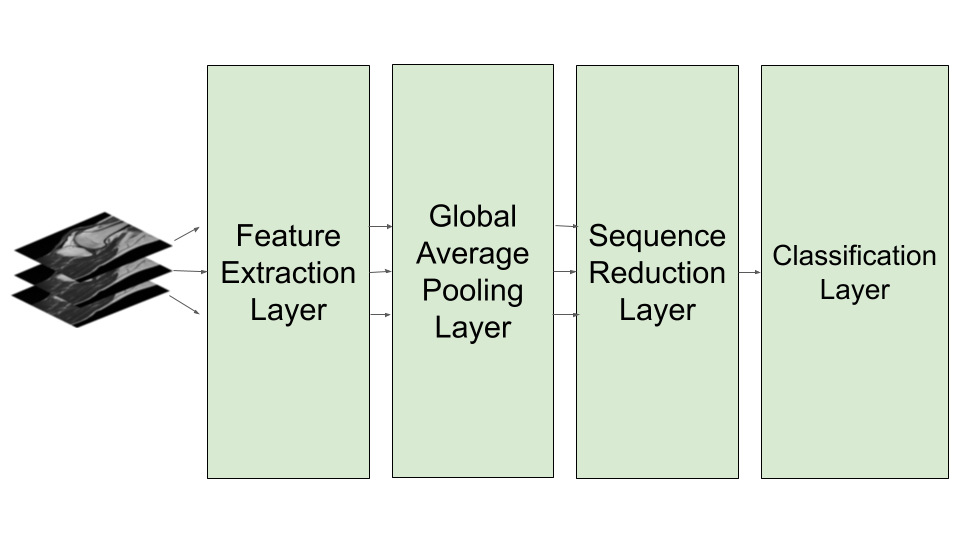
\includegraphics[width=0.6\linewidth]{../images/diagram/network2.png}
\end{center}
   \caption{An abstract view of the sequence-specific networks. Image of a knee MRI taken from \cite{knee-image}.}
\label{fig:network}
\end{figure}

\section{Methods}

\subsection{Sequence Network}

In Figure \ref{fig:network}, we illustrate an abstract procedure for transforming a single MRI sequence into an injury prediction. On the left-hand side of the diagram, a set of $n$ images, each represented as a $\mathbb{R}^{3 \times 224 \times 224}$ tensor, is inputted into the network as a unified batch. The feature extractor then transforms each of these images into a $\mathbb{R}^{c \times w \times h}$ tensor, where $c$ signifies the channel count, while $w$ and $h$ denote the width and height, respectively. These resulting features are subsequently converted into a sequence of $\mathbb{R}^c$ vectors through the global average pooling layer. Finally, the complete batch of $n$ vectors is condensed into a single $\mathbb{R}^c$ vector within the sequence reduction layer. This vector undergoes further processing via a linear layer and a sigmoid activation function in the classification layer, ultimately yielding a probability estimate regarding whether the entire MRI sequence signifies the presence of the specified injury.

Concretely, if we describe the feature extraction layer as a function, $f: \mathbb{R}^{n \times 3 \times 244 \times 244} \rightarrow \mathbb{R}^{n \times c \times w \times h}$, and the sequence reduction layer as a function $g: \mathbb{R}^{n \times c} \rightarrow \mathbb{R}^c$, then the entire network can be written as:

$$ gap_c(x^{(i)}) = \frac{\sum_{j=1}^w \sum_{k=1}^h x_{c,j,k}^{(i)}}{wh} $$

\begin{equation}
\label{eq:network}
p = \sigma(g(gap(f(x))) W_c + b_c)
\end{equation}

where $p$ is the predicted probability, $W_c \in \mathbb{R}^{c \times 1}$ and $b_c \in \mathbb{R}^c$ are the weights and biases of the classification layer and $\sigma$ is the sigmoid function: $\frac{1}{1 + e^{-x}}$

The current state-of-the-art system, MRNet - which was discussed in detail in Section \ref{related-work}, can be described as using parts of a pretrained AlexNet for the feature extraction layer, and an element-wise maximum to flatten the sequence in the sequence reduction layer.

\subsection{SqueezeNet}


\begin{figure}
\begin{center}
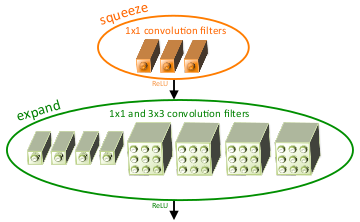
\includegraphics[width=0.6\linewidth]{../images/fire/fire.png}
\end{center}
   \caption{Illustration of a fire layer. Image taken directly from ``SqueezeNet: AlexNet-level accuracy with 50x fewer parameters and $<$0.5 MB model size''\cite{iandola2016squeezenet}}
\label{fig:fire}
\end{figure}

SqueezeNet is a convolutional neural network that achieves high performance on the ImageNet challenge. It is composed of a series of ``fire'' layers, each of which consists of a layer of $1 \times 1$ convolutional filters (the squeeze layer), followed by a ReLU and then a mix of $1 \times 1$ and $3 \times 3$ convolutional layers (the expand layer) whose outputs are concatenated before going through a final ReLU activation. An illustration of a fire layer is shown in Figure \ref{fig:fire}. These layers are interspersed with max pooling layers before the 1st, 4th, and 8th fire layers, and the entire network begins with a traditional $7 \times 7$ convolutional layer.

Fine-tuning a SqueezeNet model that has been pretrained on the ImageNet data set is a method that has been used successfully to classify vehicles\cite{agoes2017fine}, crop disease\cite{durmucs2017disease}, and cataracts\cite{qian2018machine}. By removing the final dropout, convolution, ReLU and average pooling layers from the pretrained network, we can use it as a drop-in replacement for the feature extraction layer in Figure \ref{fig:network}.

\subsection{Attention}
Attention is a mechanism that has traditionally been applied as a summarization method of the hidden states in a recurrent neural network. Given one or more queries $\textbf{Q} \in \mathbb{R}^{1 \times d}$, a set of keys $\textbf{K} \in \mathbb{R}^{n \times d}$, and a set of values $\textbf{V} \in \mathbb{R}^{n \times d}$, the attention score can be calculated as the softmax of the dot product between the query and keys:

$$s = (\textbf{Q}\textbf{K}^T)$$
$$a_i = \frac{e^{s_i}}{\sum_{j=1}^k e^{s_j}}$$
 as described by Tan, et al.\cite{tan2018deep}, whose work was derived from Luong et. al's location-based attention\cite{luong2015effective}. The attention scores can then be used as if they were weights for a weighted average of the values, $\textbf{V}$.

In the case of an RNN, the query is often the final hidden state, the keys are either the input embeddings or the hidden states at each time step, and the values are the hidden states at each time step. A final representation of the entire sequence is generated by taking the dot product the attention vector and the values, $a \textbf{V}$.

For the experiments in this paper, we eschew the use of an RNN and simply use the attention-weighted average across frames of the MRI sequence to generate the final representation of the sequence. In this case, the query is a learned parameter of the network, $\textbf{Q} \in \mathbb{R}^{1 \times c}$, while both the keys and values are taken from the output of the global average pooling layer, $\mathbb{R}^{s \times c}$. This allows us to use the attention-weighted sum as the sequence-reduction layer:

$$ \textbf{K} = \textbf{V} = gap(f(x))$$
$$ g(x) = softmax(\textbf{Q} k^T) \textbf{V}$$


\subsection{Sequence Ensembling}


\begin{figure}
\begin{center}
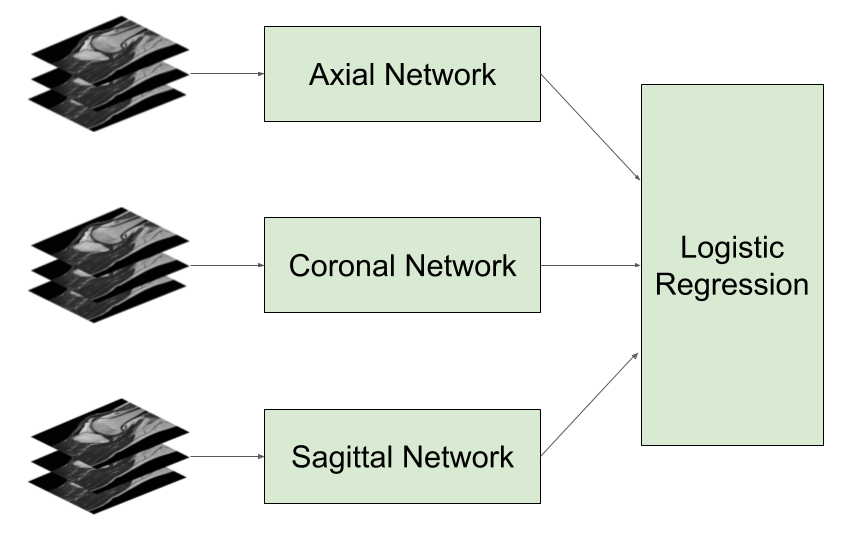
\includegraphics[width=0.8\linewidth]{../images/diagram/ensemble.png}
\end{center}
   \caption{Ensembling predictions from the sequence-specific networks to generate an injury prediction.}
\label{fig:ensemble}
\end{figure}

As we have access to multiple MRI sequences per patient, distinct networks tailored to each sequence can be trained to forecast the probability of a diagnosis. These individual probabilities are subsequently aggregated and inputted into a logistic regression classifier to produce the ultimate injury prediction, as illustrated in Figure \ref{fig:ensemble}.

\subsection{Model and Sequence Ensembling}
\begin{figure}
\begin{center}
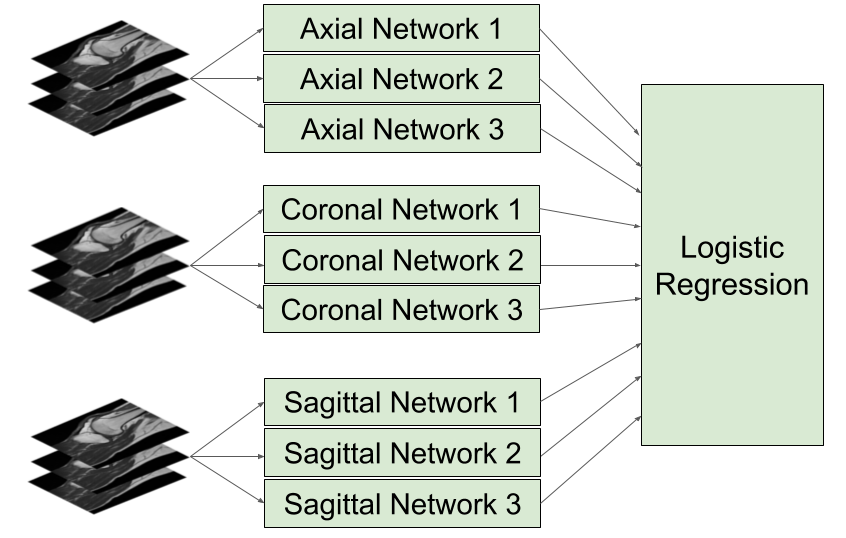
\includegraphics[width=0.8\linewidth]{../images/diagram/ensemble-of-ensembles.png}
\end{center}
   \caption{Ensembling predictions from multiple sequence-specific network types to generate an injury prediction.}
\label{fig:ensemble-of-ensembles}
\end{figure}

In addition to this per-model sequence ensembling, we can also use the sequence predictions from \textit{multiple model types} as features for a logistic regression model, as shown in Figure \ref{fig:ensemble-of-ensembles}.

\subsection{Loss}

Because of the imbalanced class sizes in the data set, all of the sequence-specific models are trained with a weighted binary cross-entropy loss:

$$ L = -\frac{1}{N} \sum_{i=0}^N w_i \big(y_i log(p_i) + (1 - y_i) log(1 - p_i)\big)$$

where $w_i$ is the fraction of the instances in the data set that have label $y_i$, and $p_i$ is the output of the network described by Equation \ref{eq:network} for sequence $i$.

\section{Dataset} 

The MRI data provided in the \href{https://stanfordmlgroup.github.io/competitions/mrnet/}{MRNet challenge} contains scans from 3 MRI types (axial, coronal, and sagittal) with 3 labels per MRI (abnormality, ACL tear, and meniscal tear) for 1,250 examinations.

The released data has already been split into a training and validation set, and a test set has been withheld for leaderboard purposes. In order to evaluate the methods deployed in this paper, we have further divided the training set into training and tuning sets, and are using the validation set for all reported metrics. Counts of cases and labels for each set can be seen in Table \ref{tab:dataset}.

\subsection{Preprocessing}


The dataset is presented in the form of numpy arrays\cite{numpy}, each representing a 3-dimensional matrix corresponding to a particular sequence for each case. These matrices have already been derived from the Digital Imaging and Communications in Medicine (DICOM) files and resized to dimensions of $256 \times 256$ images.

During the training process, we perform several preprocessing steps on the input images. Firstly, we crop the images to dimensions of $224 \times 224$ to align with the expected input size of a pretrained ImageNet model. Following this, we standardize each input sequence by subtracting the minimum pixel value and then dividing by the observed range within the sequence. Subsequently, we rescale the image to fall within the pixel value range of $0-256$. Finally, we normalize the sequence data by subtracting the mean value of the dataset, which is $58.09$, and dividing it by the dataset's standard deviation, which is $49.73$.
\subsection{Augmentation}

In order to prevent overfitting the small data set, we perform data augmentation during training. Every image is randomly flipped horizontally, shifted horizontally by -25 to 25 pixels, and rotated by -25 to 25 degrees each time it is seen during training. Note that the same transformation is applied to every image in a given sequence.

\begin{table}
\begin{center}
\begin{tabular}{|lc|c|c|c|}
\hline
Diagnosis & Label & Training & Tuning & Validation \\
\hline
\multirow{ 3}{*}{Abnormal} & Positive & 835 & 78 & 95 \\
                           & Negative & 175 & 42 & 25 \\
                           & Total & 1010 & 120 & 120 \\
\hline
\multirow{ 3}{*}{ACL}      & Positive & 167 & 41 & 54 \\
                           & Negative & 843 & 79 & 66 \\
                           & Total & 1010 & 120 & 120 \\
\hline
\multirow{ 3}{*}{Meniscus} & Positive & 353 & 44 & 52 \\
                           & Negative & 657 & 76 & 68 \\
                           & Total & 1010 & 120 & 120 \\
\hline
\end{tabular}
\end{center}
\caption{MRNet data splits and label counts.}
\label{tab:dataset}
\end{table}

\section{Experiments} 
\begin{table}
\begin{center}
\begin{tabular}{|l|c|c|}
\hline
Name & Feature Extraction Layer \\
\hline
MRNet & AlexNet \\
MRNet-Squeeze & SqueezeNet \\
MRNet-Attend & AlexNet \\
MRNet-SqueezeAttend & SqueezeNet \\
\hline
\end{tabular}
\end{center}
\caption{Model combinations used in experiments.}
\label{tab:models}
\end{table}

\begin{table}
\begin{center}
\begin{tabular}{|l|c|c|}
\hline
Sequence Reduction Layer \\
\hline
Max pooling \\
Max pooling \\
Attention \\
Attention \\
\hline
\end{tabular}
\end{center}
\caption{Model combinations used in experiments.}
\label{tab:models}
\end{table}

Referring to the abstract network image shown in Figure \ref{fig:network}, Table \ref{tab:models} shows the combinations of feature extraction and sequence reduction techniques used in the experiments in this paper. In each case, a pretrained network that was tuned on ImageNet was used to extract features. The pretrained network was fine-tuned on the MRNet data along with the other layers of the model.

In addition to these models, we include results from ensembling the sequence-specific predictions of all four models, as described in Figure \ref{fig:ensemble-of-ensembles}.

\begin{table}
\begin{center}
\begin{tabular}{|l|l|}
\hline
Optimization Method & Adam \\
Weight Decay & 0.01 \\
\hline
Learning Rate Schedule & Reduce on plateau \\
Initial Learning Rate & 0.00001 \\
Max Patience & 5 \\
Factor & 0.3 \\
\hline
Max Epochs & 40 \\
\hline
Logistic Regression Penalty & L2 \\
Logistic Regression Lambda & 1.0 \\
\hline

\end{tabular}
\end{center}
\caption{Hyperparameters for all experiments.}
\label{tab:hyperparams}
\end{table}

Table \ref{tab:hyperparams} shows the hyperparameters used for all experiments. Most of these hyperparameters were drawn from the original MRNet paper, although Initial Learning Rate and Max Epochs were determined with brief experiments on the axial sequence and abnormal label. Due to the processing time required to run these models, extensive hyperparameter optimization was not feasible, although this would be a potential area for future work.

\section{Results}
The primary evaluation metric employed for model comparison is the Area Under the ROC Curve (AUC). To derive a comprehensive metric for each model, the AUC scores for the three distinct labels are averaged. Furthermore, we present the specificity, sensitivity, and accuracy for all four models and the ensemble concerning each label. This assessment involves utilizing a threshold of $0.5$ to transform probabilities into label predictions.

Table \ref{tab:results} shows the AUC for each model on each injury prediction, as well as averaged across all injuries. Each of the individual model types perform well on some of the injury categories, but none of them excel at all injuries. For detecting any kind of abnormality, the original MRNet implementation gets the highest AUC $(0.940)$. MRNet-Squeeze is the best model for detecting ACL injuries $(0.974)$, while MRNet-SqueezeAttend achieves the highest AUC on the Meniscal tear category $(0.885)$.

By using all four model types together, however, we can capture that varying performance on the three injuries to create an ensembled model that outperforms any of the individual models. The ensembled model achieves nearly the highest AUC on all individual injury types, and significantly outperforms the others with an average AUC of $0.931$.

MRNet (reported) is the AUC reported by Bien, et al.\cite{bien2018deep}, and is not directly comparable to the values shown here because the released data is a subset of the data used in their experiments.

\begin{table}[h!]
\begin{center}
\begin{tabular}{|l|c|c|c|c|}
\hline
Model & Average & Abnormal & ACL & Meniscus \\
\hline
MRNet (reported) & 0.916 & 0.937 & 0.965 & 0.847 \\
\hline
MRNet & 0.913 & \textbf{0.940} & 0.960 & 0.839 \\
MRNet-Squeeze & 0.910 & 0.925 & 0.974 & 0.829 \\
MRNet-Attend & 0.891 & 0.925 & 0.910 & 0.838 \\
MRNet-SqueezeAttend & 0.915 & 0.936 & 0.925 & \textbf{0.885}\\
\hline
Ensemble & \textbf{0.931} & 0.939 & \textbf{0.976} & 0.876 \\
\hline
\end{tabular}
\end{center}
\caption{AUC on the validation set}
\label{tab:results}
\end{table}

Table \ref{tab:metrics} shows the specificity, sensitivity, and accuracy of each model, as well as the human performance of expert radiologists, as reported by Bien et al.\cite{bien2018deep}. Once again, the experiments in this paper are not directly comparable to the reported human values because of differing data sets, especially on these metrics since class imbalance can have an outsized effect on precision and recall. On these metrics, the final ensemble achieves state of the art on some injury types and not others.

\begin{table}[h!]
\begin{center}
\begin{tabular}{|l|c|c|c|}
\hline
Prediction & Specificity & Sensitivity & Accuracy \\
\hline
\multicolumn{4}{l}{\textbf{Abnormality} }\\
\hline
Radiologist & 0.844 & 0.905 & 0.894 \\
MRNet (reported) & 0.714 & 0.879 & 0.850 \\
\hline
MRNet & 0.440 & 0.968 & 0.858 \\
MRNet-Squeeze & 0.560 & 0.968 & 0.883 \\
MRNet-Attend & 0.480 & 0.979 & 0.875  \\
MRNet-SqueezeAttend & 0.440 & 0.968 & 0.858 \\
\hline
Ensemble & 0.480 & 0.958 & 0.858 \\
\hline
\multicolumn{4}{l}{\textbf{ACL tear} }\\
\hline
Radiologist & 0.933 & 0.906 & 0.920 \\
MRNet (reported) & 0.968 & 0.759 & 0.867 \\
\hline
MRNet & 0.894 & 0.907 & 0.900 \\
MRNet-Squeeze & 0.909 & 0.963 & 0.933 \\
MRNet-Attend & 0.803 & 0.778 &  0.792 \\
MRNet-SqueezeAttend & 0.864 & 0.852 & 0.858 \\
\hline
Ensemble & 0.909 & 0.981 & 0.942 \\
\hline
\multicolumn{4}{l}{\textbf{Meniscus tear} }\\
\hline
Radiologist & 0.882 & 0.820 & 0.849 \\
MRNet (reported) & 0.741 & 0.710 & 0.725 \\
\hline
MRNet & 0.721 & 0.788 & 0.750 \\
MRNet-Squeeze & 0.735 & 0.731 & 0.733 \\
MRNet-Attend & 0.691 & 0.846 &  0.758 \\
MRNet-SqueezeAttend & 0.794 & 0.750 & 0.775 \\

\hline
Ensemble & 0.735 & 0.865 & 0.792 \\
\hline
\end{tabular}
\end{center}
\caption{Metrics on the validation set}
\label{tab:metrics}
\end{table}

\begin{figure}[h!]
\begin{center}
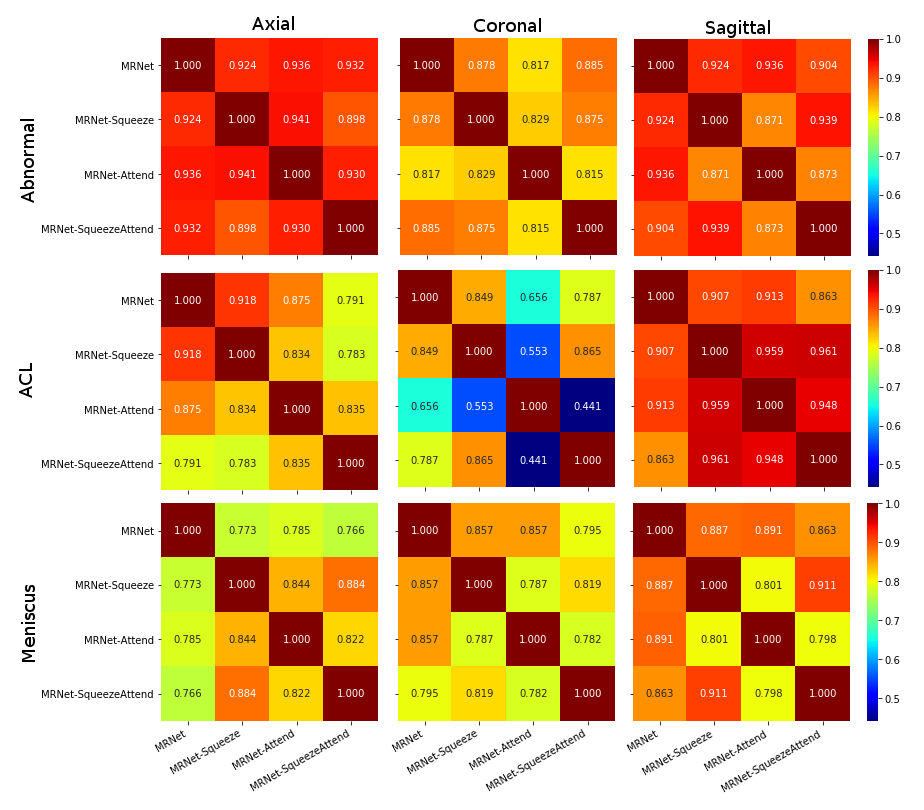
\includegraphics[width=0.9\linewidth]{../images/corr2/corr2.png}
\end{center}
   \caption{Correlation between sequence-specific predictions on the validation set.}
\label{fig:corr}
\end{figure}



It is interesting to consider the differences between the four models, especially at the level of the sequence-specific predictions (i.e. the values that get fed into the logistic regression classifier). If the sequence-specific predictions from each individual model are highly correlated, then we would not expect the multi-model ensemble to outperform the individual models. Figure \ref{fig:corr} shows the correlation between the sequence-specific predictions on the validation set for the four models. There is a strong correlation between the models' sequence-specific predictions on some diagnosis/sequence combinations (for instance, Abnormal/Axial and ACL/Sagittal), but on other combinations the correlation is quite low (ACL/Coronal, Meniscus/Axial). These areas of low correlation are likely useful signals for the multi-model ensemble.

\begin{table}[h!]
\begin{center}
\begin{tabular}{|l|l|}
\hline
Model & Frame \\
\hline
MRNet & 11 \\
MRNet-Squeeze & 7 \\
MRNet-Attend & 20 \\
MRNet-SqueezeAttend & 6 \\
\hline
\end{tabular}
\end{center}
\caption{The most focused on frame of the axial sequence for each model when predicting whether Case 1218 has an ACL tear.}
\label{tab:frames}
\end{table}

Another way to look at the differences between models is to examine, for a particular diagnosis/sequence combination, what areas of the MRI each model is focusing on. If we consider a specific instance in the validation set, Case 1218, and look at a specific diagnosis/sequence pair, ACL/Axial, we can ask which image from the sequence each model is most interested in. For the models that use attention (MRNet-Attend and MRNet-SqueezeAttend) that simply means asking for the argmax of the calculated attention vector. For MRNet and MRNet-Squeeze, the sequence reduction layer takes the maximum value over the sequence for each location in the features vector. For those models, we can say that the frame with the most maximum values is the one that the model is ``most interested'' in. Table \ref{tab:frames} shows the most interesting frame of the axial sequence for each model when asked to predict whether Case 1218 has an ACL tear.

We can go further though, and examine the class activation map (CAM) for each of those frames for each model. A class activation map is a way of visualizing where in the image a model is focusing its (implicit) attention\cite{zhou2016learning}. To calculate the CAM for the frames listed in Table \ref{tab:frames}, we use $W_c$ from Equation \ref{eq:network} to compute a weighted average of the $c$ feature maps (each feature map $\in \mathbb{R}^{w \times h}$) generated by running the single frame through the feature extraction layer of the sequence-specific model. That is, let $F$ be the $\mathbb{R}^{c \times w \times h}$ tensor returned by running a frame through the feature extraction layer. Then we calculate an image $I \in \mathbb{R}^{w \times h}$:

$$I_{i,j} = \frac{1}{c} \sum_{a=1}^c W_{c_a} F_{i, j}$$

By scaling this image up to the original MRI image size $(256 \times 256)$ and using the values as a colormap to overlay on the image, we can create a visualization of where the model's attention is focused for each frame. Figure \ref{fig:cam_4x4} shows the CAM for the four models (across the columns) for the 11th, 7th, 20th, and 6th frame, i.e. each model's ``most interesting'' frame (across the rows).

\begin{figure}[h!]
\begin{center}
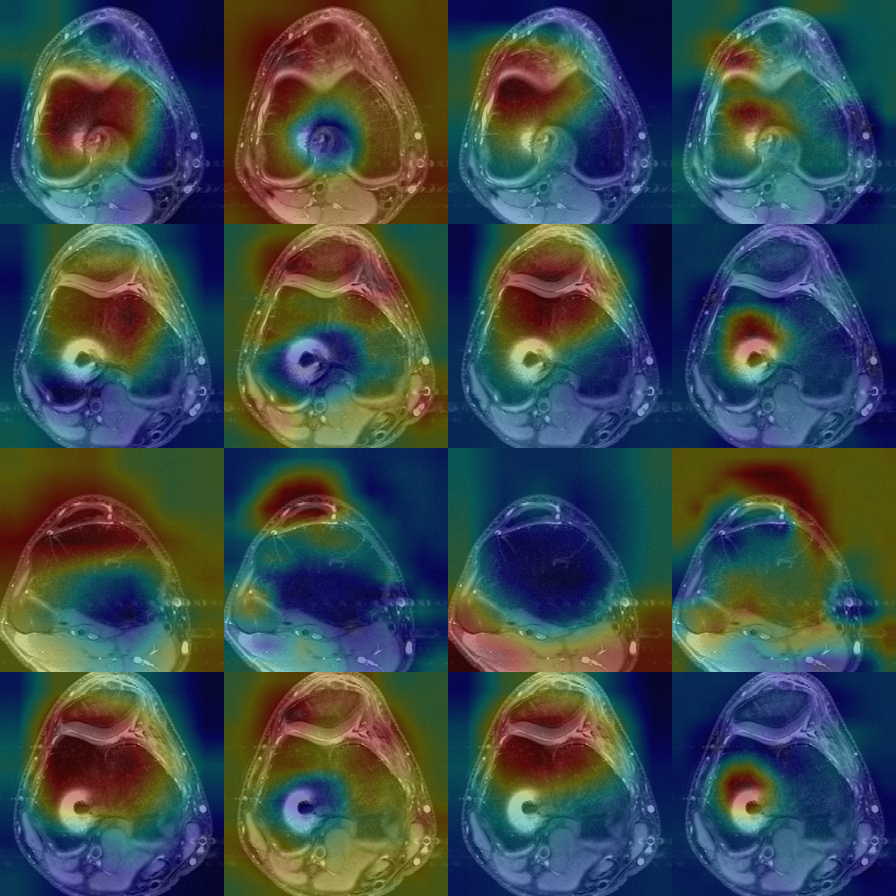
\includegraphics[width=0.9\linewidth]{../images/cams/4x4.png}
\end{center}
   \caption{Class activation maps from the four networks for the axial sequence of Case 1218, when asked to predict whether there is an ACL tear. From left to right, the columns are class activation maps for MRNet, MRNet-Squeeze, MRNet-Attend, and MRNet-SqueezeAttend. Each row represents the frame from the axial sequence that each network found most interesting.}
\label{fig:cam_4x4}
\end{figure}


\section{Conclusion/Future Work} 

The experiments in this paper use transfer learning to predict injury diagnoses from MRI sequences of the knee. We compare pretrained AlexNet and SqueezeNet models as feature extractors and max pooling versus attention mechanisms to reduce the information across the sequence. Finally, we use a logistic regression, trained on the sequence-specific predictions, to predict the probability of the diagnosis for the patient.

We show that all of the models have different strengths and weaknesses, some achieving higher AUC scores than others on each diagnosis. Furthermore, we show that by ensembling not just different sequence predictions, but multiple sequence predictions from multiple sequence models, we can outperform the current state of the art on the MRNet data set.

There is still a lot left to explore here though. Future work should include examining how to get greater diversity in the sequence-specific models. Some possibilities for decreasing the correlation between predictions are:
\begin{itemize}
\item Using other pretrained feature extractors in the Feature Extraction layer.
\item Swapping the order of the Global Average Pooling layer and the Sequence
Reduction layer.
\item Using more advanced methods like RNNs in the Sequence Reduction layer.
\end{itemize}

We also believe that there is a possibility of using inter-sequence attention to compute a final representation of all three sequences, but exploring that was beyond the scope of this project. Finally, an end-to-end ensemble model, instead of using logistic regression on the sequence-specific predictions, may lead to more robust models.

\subsection{Failed Experiments}
We briefly tried some of the next steps mentioned above, but was not able to achieve AUC scores as high as any of the individual models, much less the final multi-model ensemble. With more time, any one of these paths could be useful.

Specifically, we tried:
\begin{itemize}
   \item Using a pretrained ResNet in place of AlexNet or SqueezeNet. Despite many attempts at freezing or removing various layers and adding dropout, we were not able to prevent models with this feature extractor from overfitting on the sequence-specific predictions.
   \item Using pretrained DenseNet or VGG in place of AlexNet or SqueezeNet. DenseNet and VGG both require significantly more memory than the other networks, which prevented us from using them since the model architecture requires passing all of the frames in an MRI sequence through at once.
   \item Using LSTM and BiLSTM layers in place of max pooling or attention in the Sequence Reduction layer. Here we struggled with underfitting, even with more LSTM layers.
   \item Training end-to-end networks instead of ensembling the sequence-specific predictions. We believe that these networks were overfitting. The average AUC scores ranged from 0.860 (MRNet-SqueezeAttend) to 0.889 (MRNet).
\end{itemize}

\bibliographystyle{IEEEtran}
\bibliography{egbib}

\end{document}
